\documentclass[0-suturing.tex]{subfiles}
\begin{document}

\section{System Design}
\label{sec:system}
\subsection{User Interface for wound tracing.}
describe the simple interface here

 dVRK is a research platform built from mechanical components from the first-generation of the \davinci surgical system \cite{Ballantyne2003} and electronics and software from WPI and Johns Hopkins University~\cite{Kazanzides2014}.

\subsection{Multilateral Hand-offs for Optimal Needle Re-orientation}
describe the search method here.  


\subsection{Needle Tracking}
Block diagram for the approach along with real images. 
some explanation of the math, and cite CPD2 for affine point registration. 
step by step.

Needle Tracking

    We use paint to color our needles yellow so that we can use HSV thresholding to
segment the needles. We apply an erosion filter to the image to remove noise and
outlier pixels from segmented image. Next we use point set registration to fit an
elliptical arc to the segmentation mask. We use the CPD2 algorithm to find
an affine transformation which when applied to a circular arc, best fits our
segmentation. This process in repeated in our left and right camera images and
correspondence points are used to generate 3D points along the needles.
The end points are used to generate a pose on the the left and right edges of
the needle. We apply a kalman filter to smooth our pose estimates.
Our needle alignment tool tips ensure that the needles lie on a known plane when
they are held by the grippers. We project our gripper estimates onto this known
plane to improve the robustness our estimates.
    Since the point set registration algorithm is robust to outliers and missing
data, the needle can still be tracked in instances when it is partially oclluded.
Partial ocllutions occur whenever the needle is being held in a tool or when it
is inserted into tissue. Both are instances when needle tracking is necessary
for closed loop control. Furthermore, specularies and changes in lighting conditions
cause cause the HSV segmentation to be incomplete - resulting in needle masks
containing holes. Our technique allows us to interpolate points along the needle
in these holes.




\begin{figure}[!t]
\centering
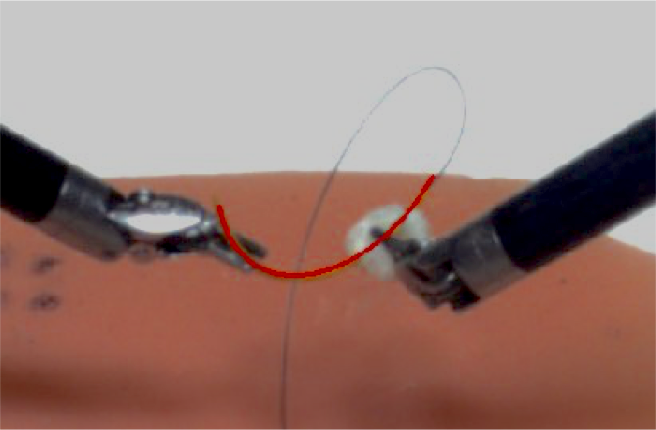
\includegraphics[width=0.9\linewidth]{figures/needleTrack}
% \vspace{-5pt}
\caption{\todo{Placeholder}The figure illustrates our needle tracking system along with the algorithm used. This system can successfully track needle pose through partial occlusions such as when needle is parially inside tissue and gripper occlusions during hand-offs.}
\label{fig:tracking}
\vspace{-10pt}
\end{figure}


\subsection{Design of a Needle Driver Jaw Attachment to Facilitate Pose Orientation}

A difficulty faced in the automation of suturing is the uncertainty of needle pose \tocite. Position and orientation of a needle gripped within the \textit{da~Vinci Large Needle Driver} is unconstrained for rotation in two directions and translation along the length of the needle. Although perception of a needle within a surgical workspace is possible using stereoscopic vision \tocite, it is still noisy and uncertain \tocite. Even with perfect perception, additional time consuming steps would be needed to correct the needle's pose. Constraining the orientation of a grasped needle to a single degree of freedom would allow for easier pose estimation as well as fewer pass-offs. Based off of previous work in self righting grippers such as \cite{Articulating needle driver} and 
\cite{Needle holder with suture filament grasping abilities}, the needle gripper attachment was designed to orient a curved needle to a single pose with uncertainly only in translation along the length of the needle. As the grippers approach a needle, the needle is funneled towards a groove running perpendicular to the length of the gripper jaws. Upon closing the jaws, the needle rolls to a single pose of stability between contact points C \todo{add contact points C and J to figure} and jaw J as shown in Figure~\todo{add figure reference}(b) and Figure~\todo{add figure ref}(d).



The front plane of the jaw attachment (area P \todo{add area P to figure} in Figure~\todo{add figure ref}(c)) is designed to provide a collision surface for the approaching needle and is also used as a mechanical constraint for a second Needle Driver during the process of needle passing. The rear wall R shown in Figure~\todo{refer to figure}(a) \todo{add R to figure} is designed to provide a collision surface for an approaching needle. These features (area P and wall R) are designed to overcome needle and Needle Driver pose uncertainty and passively facilitate needle gripping and pose estimation. The size of the needle gripper and the distance between contact points P is dependent on the curvature of the needle; in this case, we designed our gripper specifically for the ½ 36mm needle, resulting in a total width of 10mm.

We fabricated the mount out of ABS plastic using a Stratysys uPrint 3D printer. Due to surface texture of the $3$D-printed surface and the triangular cross-section of the needle, a semi-stable antipodal pose can be achieved if the needle is initially approached 180 degrees from its desired pose. Kinematic or visual feedback can be used to determine if this has occurred, and a re-grasp can be attempted produce the desired results.

\todo{flesh out the second version of design, why is it concave not convex --rather counter intuitive, }

\begin{figure}[t!]
\centering
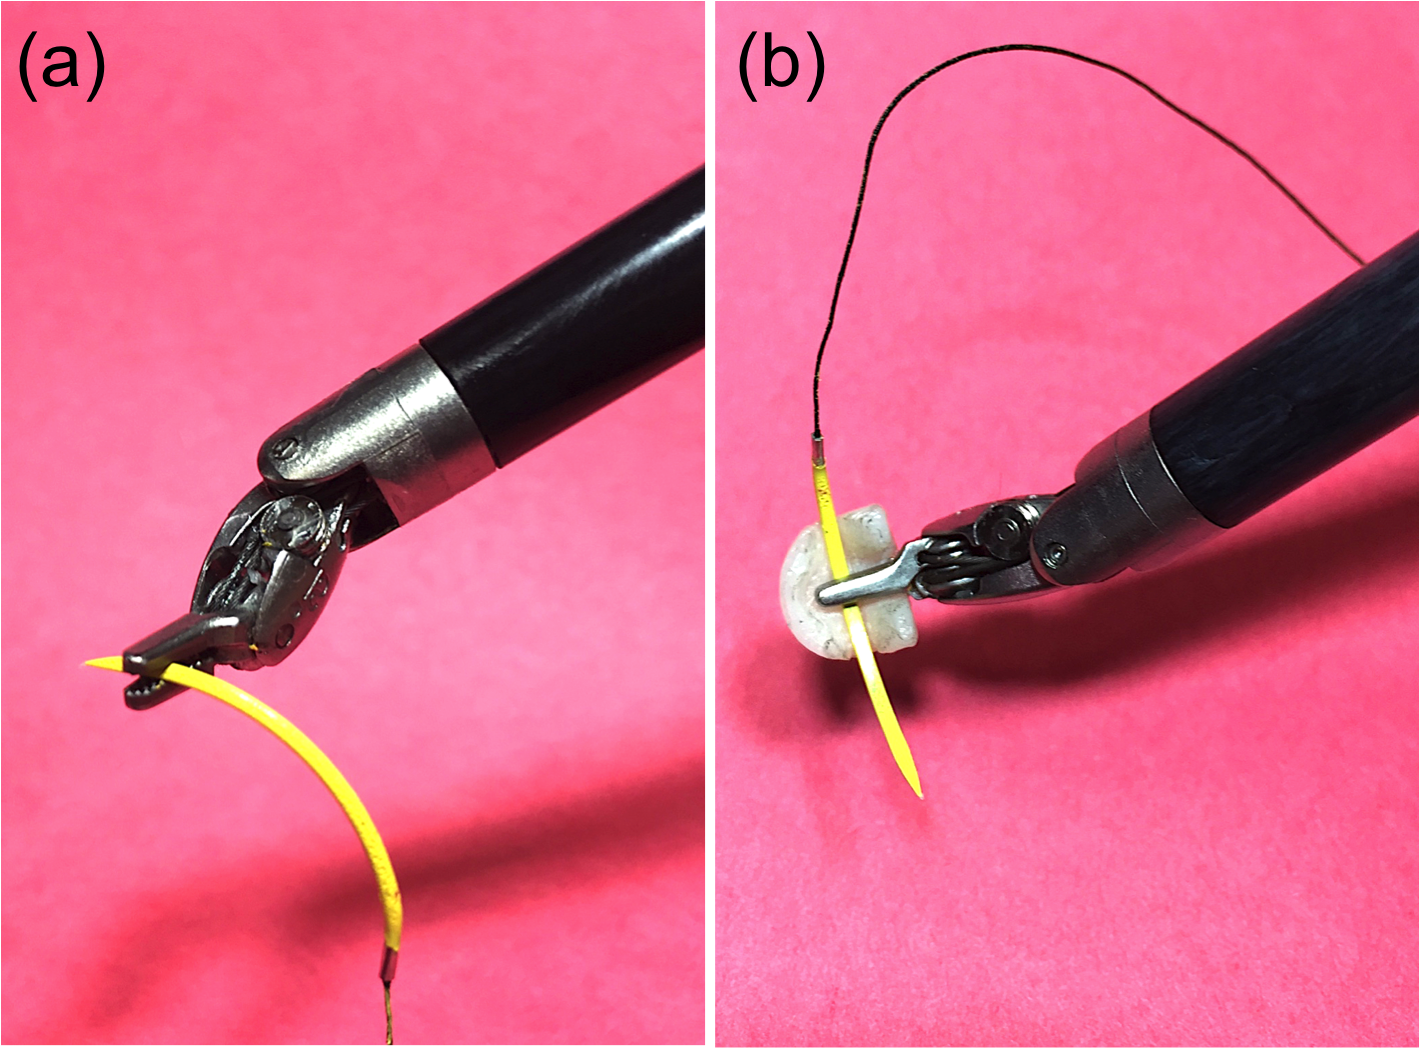
\includegraphics[width=0.95\linewidth]{figures/gripperAttachment}
% \vspace{-5pt}
\caption{\todo{placeholder caption}Figure (a) shows a suboptimal needle orientation both in position and rotation. Figure (b) shows the passive correction in action, with the needle held in correct orientation and position to facilitate insertion. }
\label{fig:jawMount}
\vspace{-10pt}
\end{figure}


\begin{figure*}[!t]
\centering
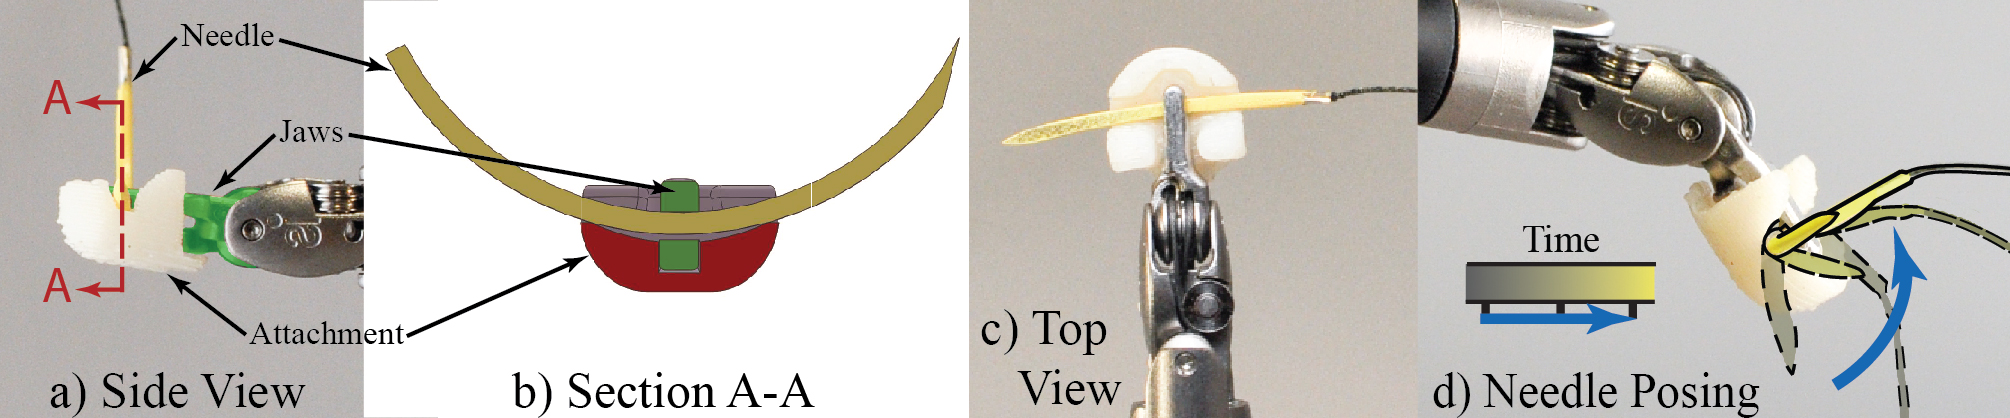
\includegraphics[width=\linewidth]{figures/NeedleGripper2-01}
% \vspace{-5pt}
\caption{\todo{caption}Detail the design of the gripper attachment}
\label{fig:gripper design}
\vspace{-10pt}
\end{figure*}

\subsection{Needle grasp and Pull Through}
describe the strategy in detail. 

\end{document}
